\documentclass[11pt, oneside]{article}   	% use "amsart" instead of "article" for AMSLaTeX format
\usepackage{geometry}                		% See geometry.pdf to learn the layout options. There are lots.
\geometry{letterpaper}                   		% ... or a4paper or a5paper or ... 
\usepackage[parfill]{parskip}    		% Activate to begin paragraphs with an empty line rather than an indent
\usepackage{graphicx}				% Use pdf, png, jpg, or eps§ with pdflatex; use eps in DVI mode
								% TeX will automatically convert eps --> pdf in pdflatex		
\usepackage{amssymb}
\usepackage{amsmath}
\usepackage{amsthm}

\usepackage{tikz}
\usetikzlibrary{decorations.pathreplacing}

\usepackage{float}
\usepackage{titlesec}
\newcommand{\sectionbreak}{\clearpage}

\usepackage{apacite}
\usepackage{url}

\linespread{1.25}

\usepackage{titling}
\renewcommand\maketitlehooka{\null\mbox{}\vfill}
\renewcommand\maketitlehookd{\vfill\null}

\theoremstyle{definition}
\newtheorem{example}{Example}[section]

\newtheorem{theorem}{Theorem}
\renewcommand{\qedsymbol}{}

\usepackage{scrextend}

\numberwithin{figure}{section}

\title{Investigation on mathematical method used to construct curves in computer systems}
\author{Daekun Kim}
%\date{}							% Activate to display a given date or no date

\begin{document}
\begin{titlingpage}
\maketitle
Word count: 1447
\end{titlingpage}
\tableofcontents
\newpage

%==========================================================================================
%==========================================================================================
%=================================== INTRODUCTION =========================================
%==========================================================================================
%==========================================================================================
\section{Introduction}
In the modern era, computer is one of the tools that are having the most influence in our lives. It is commonly used to design different products, such as cars and airplanes, or in the movie industry, such as producing scenes with computer graphics and animations. In these fields, ability to form and display smooth, realistic curvatures is essential. However, computers are digital, and they can only process discrete information. This nature of computers makes it seem to be only able to render discrete and pixelated shapes that cannot imitate natural curves. Yet, they seem to be able to easily generate many kinds of curved lines and surfaces, as shown in many computer-generated animations and products produced by computer-controlled machineries. This provoked my interest in how mathematics may play a role in achieving such seemingly impossible task.

This paper aims to investigate the mathematics behind how a computer system generates smooth curves. One of the most prominent methods used to achieve this is the \emph{B\'{e}zier curve}. It is used in many popular photo-editing and animating softwares, such as the Adobe Flash\textregistered, Blender\texttrademark, Autodesk Maya\textregistered, and more (\citeNP{MAYA:2017}; \citeNP{ADOBEF:2017}). This paper aims to clarify the journey that it took to come into being and be widespread to be utilized in numerous fields. Specifically, this paper describes the mathematical development of the B\'{e}zier curve, which starts from a rudimentary linear interpolation, repeated linear interpolation, the De Castaljau Algorithm, and finally the B\'{e}zier curve itself. Then, the properties of the B\'{e}zier curve that made it to be one of the most popular tool in curvature rendering in computer systems will be investigated.

%==========================================================================================
%==========================================================================================
%=================================== LINEAR INTERPOLATION =================================
%==========================================================================================
%==========================================================================================

\section{Linear Interpolation}

Straight lines are one of the easiest shapes one can imagine and draw, because of their simplicity to understand and manipulate. Such holds true even for computers. Graphically, drawing straight lines is the most rudimentary job a computer can perform. However, because it is so easy to render, it forms the fundamentals of how computers can render sophisticated curves and surfaces onto a screen.

Lines can be thought of as the shortest path that connects two points. A {\em linear interpolation}, then, is calculating which position on the line one would arrive on if one was to travel certain distance or time. Mathematically, given two points, \((x_0, y_0)\) and \((x_1,y_1)\) with \(x_0 < x_1\), a linear interpolation is construction of a new set of \(y\) from \(x\) values within \([x_0, x_1]\). The formula of linear interpolation can be given as a relationship of the slopes of the lines connecting the starting and end point with that of line connecting the interpolated point with the starting point, or

\begin{equation}
\frac{y-y_0}{x-x_0}=\frac{y_1-y_0}{x_1-x_0}
\end{equation}

Eq. (1) is stating that, if a person was to travel over a line, the ratio of the distances at which one travelled vertically over the horizontal distance travelled must be the same no matter the position he or she lies on the line.

\begin{quote}
\begin{example} Fig. 2.1 shows an example of linear interpolation between \((1,1)\) and \((3,2)\).

\begin{figure}[h]
	\centering
	\begin{tikzpicture}[scale=1.5]
		\draw [->] (0,0) -- (0,3) node[align=left, right] {\(y\)};
		\draw [->] (0,0) -- (4,0) node[align=left, above] {\(x\)};
		\draw (0,0) node[anchor=north east,fill=white] {0};
		\foreach \x/\xtext in {1, 2, 3} 
			\draw (\x,1pt) -- (\x,-1pt) node[anchor=north,fill=white] {$\xtext$};
		\foreach \y/\ytext in {1, 2} 
			\draw (1pt,\y) -- (-1pt,\y) node[anchor=east,fill=white] {$\ytext$};
		
		\path	(1,1) node(p0) {} 
			(3,2) node(p1) {};
		\draw (p0) -- (p1);
		\filldraw (p0) circle (1pt) node[align=center, below] {\(P_0(1,1)\)};
		\filldraw (p1) circle (1pt) node[align=center, above] {\(P_1(3,2)\)};
	\end{tikzpicture}
	\caption{Linear interpolation between two points}
\end{figure}

The equation of linear interpolation in Fig. 2.1 can be defined as following:

\begin{equation}
\frac{y-1}{x-1}=\frac{2-1}{3-1},1 \leq x \leq 2
\end{equation}

The line shown in Fig 2.1 is called the \textbf{interpolant}, which can be thought of, literally, as a shortest path between two points. Solving Eq. (2) for \(x\) gives us the following:

\begin{displaymath}
y=\frac{1}{2}(x-1)+1,
\end{displaymath}
\begin{equation}
y=\frac{1}{2}x+\frac{1}{2}
\end{equation}

In fact, this is now in slope-intercept form of an equation of a linear function, \(y=mx+b\)! This signifies that linear interpolation is nothing more than a linear function with a restricted domain between two points.

\end{example}
\end{quote}


\section{Parametric Equations}
The previous section showed that linear interpolation is essentially plotting a point on a line using a linear function. However, such is not possible with our original definition of linear interpolation when the line cannot be defined using a function. For instance, consider a straight vertical line as shown in Fig 3.1.

\begin{figure}[h]
	\centering
	\begin{tikzpicture}[scale=1.5]
		\draw [->] (0,0) -- (0,4) node[align=left, right] {\(y\)};
		\draw [->] (0,0) -- (4,0) node[align=left, above] {\(x\)};
		\draw (0,0) node[anchor=north east,fill=white] {0};
		\foreach \x/\xtext in {1, 2, 3} 
			\draw (\x,1pt) -- (\x,-1pt) node[anchor=north,fill=white] {$\xtext$};
		\foreach \y/\ytext in {1, 2, 3} 
			\draw (1pt,\y) -- (-1pt,\y) node[anchor=east,fill=white] {$\ytext$};
		
		\path	(2,1) node(p0) {} 
			(2,3) node(p1) {};
		\draw (p0) -- (p1);
		\filldraw (p0) circle (1pt) node[align=center, below] {\(P_0(1,1)\)};
		\filldraw (p1) circle (1pt) node[align=center, above] {\(P_1(3,2)\)};
	\end{tikzpicture}
	\caption{A vertical linear interpolation}
\end{figure}

In order for a line to be defined by a function, it must pass the Vertical Line Test, which states that there can only be one and only one \(y\) value for each \(x\) value. The line shown in Fig 3.1 obviously does not pass this condition, since there are infinitely many \(y\) values for \(x=2\).

However, by redefining linear interpolation with a set of parametric equations, one can easily overcome this apparent problem. Instead of defining an interpolation in respect to \(x\), we can do so with another variable \(t\) within \([0,1]\), and define different equations for the values of \(y\) and \(x\) with no explicitly direct relationship between them. This new variable \(t\) can be thought of as the time, or the ratio of how much of the path one have travelled from the initial point.

\begin{quote}
\begin{example}

\begin{figure}[h]
	\centering
	\begin{tikzpicture}[scale=2]
		\draw [->] (0,0) -- (0,3) node[align=left, right] {\(y\)};
		\draw [->] (0,0) -- (4,0) node[align=left, above] {\(x\)};
		\draw (0,0) node[anchor=north east,fill=white] {0};
		\foreach \x/\xtext in {1, 2, 3} 
			\draw (\x,1pt) -- (\x,-1pt) node[anchor=north,fill=white] {$\xtext$};
		\foreach \y/\ytext in {1, 2} 
			\draw (1pt,\y) -- (-1pt,\y) node[anchor=east,fill=white] {$\ytext$};
		
		\path	(1,1) node(p0) {} 
			(3,2) node(p1) {};
		\filldraw (p0) circle (1pt) node[align=center, below] {\(P_0(1,1)\)};
		\filldraw (p1) circle (1pt) node[align=center, above] {\(P_1(3,2)\)};
		\draw (p0) -- (p1);
		\draw (1,1) -- (3,1);
		\draw (1,1) -- (1,2);
		\draw[dashed] (2,1) -- (2,1.5);
		\draw[dashed] (1,1.5) -- (2,1.5);
		\filldraw (2,1.5) circle (1pt) node[align=center, below right] {\(P'(2,\frac{3}{2})\)};
%		\draw (2,1+0.05) -- (2,1-0.05) node[anchor=north,fill=white] {t=0.5};
		\draw (1.46,1+0.05) -- (1.5,1-0.05);
		\draw (1.5,1+0.05) -- (1.54,1-0.05);
		\draw (2.46,1+0.05) -- (2.5,1-0.05);
		\draw (2.5,1+0.05) -- (2.54,1-0.05);
		\draw (1+0.05,1.23) -- (1-0.05,1.27);
		\draw (1+0.05,1.73) -- (1-0.05,1.77);
	\end{tikzpicture}
	\caption{Parametric linear interpolation for \(t=0.5\)}
\end{figure}

Fig. 3.2 shows a linear interpolation at \(t=0.5\). At \(t=0.5\), the resulting point at halfway between \(P_0\) and \(P_1\) in both directions of the \(x\)- and \(y\)-axes. This can be thought of as a driver having travelled 50\% of the path.
\end{example}
\end{quote}

\begin{quote}
\begin{example}

\begin{figure}[h]
	\centering
	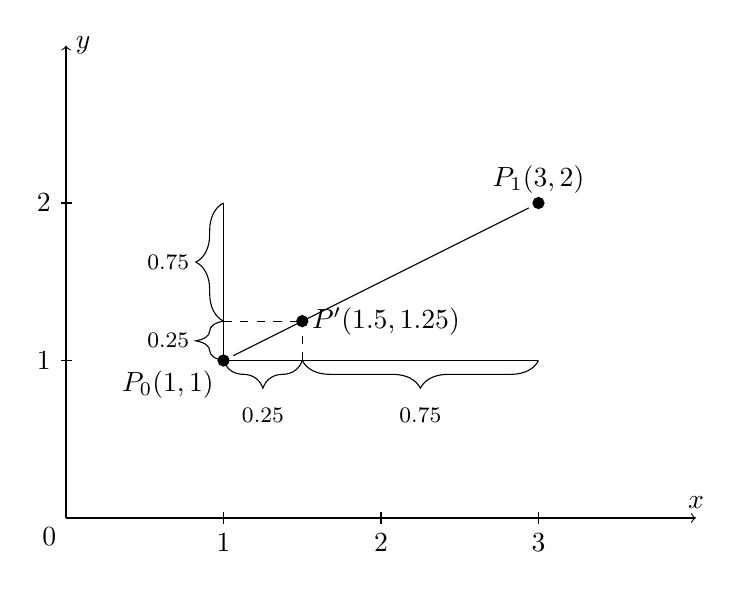
\begin{tikzpicture}[scale=2]
		\draw [->] (0,0) -- (0,3) node[align=left, right] {\(y\)};
		\draw [->] (0,0) -- (4,0) node[align=left, above] {\(x\)};
		\draw (0,0) node[anchor=north east,fill=white] {0};
		\foreach \x/\xtext in {1, 2, 3} 
			\draw (\x,1pt) -- (\x,-1pt) node[anchor=north,fill=white] {$\xtext$};
		\foreach \y/\ytext in {1, 2} 
			\draw (1pt,\y) -- (-1pt,\y) node[anchor=east,fill=white] {$\ytext$};
		
		\path	(1,1) node(p0) {} 
			(3,2) node(p1) {};
		\filldraw (p0) circle (1pt) node[align=center, below left] {\(P_0(1,1)\)};
		\filldraw (p1) circle (1pt) node[align=center, above] {\(P_1(3,2)\)};
		\draw (p0) -- (p1);
		\draw (1,1) -- (3,1);
		\draw (1,1) -- (1,2);
		\draw[dashed] (1.5,1) -- (1.5,1.25);
		\draw[dashed] (1,1.25) -- (1.5,1.25);
		\filldraw (1.5,1.25) circle (1pt) node[align=center, right] {\(P'(1.5,1.25)\)};
		\draw [decorate,decoration={brace,amplitude=10pt,mirror},xshift=0pt,yshift=0pt] (1,1) -- (1.5,1) node [black,midway,yshift=-20pt] {\footnotesize \(0.25\)};
		\draw [decorate,decoration={brace,amplitude=10pt,mirror},xshift=0pt,yshift=0pt] (1.5,1) -- (3,1) node [black,midway,yshift=-20pt] {\footnotesize \(0.75\)};
		
		\draw [decorate,decoration={brace,amplitude=10pt},xshift=0pt,yshift=0pt] (1,1) -- (1,1.25) node [black,midway,xshift=-20pt] {\footnotesize \(0.25\)};
		\draw [decorate,decoration={brace,amplitude=10pt},xshift=0pt,yshift=0pt] (1,1.25) -- (1,2) node [black,midway,xshift=-20pt] {\footnotesize \(0.75\)};
	\end{tikzpicture}
	\caption{Parametric linear interpolation for \(t=0.25\)}
\end{figure}

In the same way, at \(t=0.25\), the resulting points are one-quarter of the way between the initial and the terminal points in both axes, which is like travelling 25\% of the path since the starting point.
\end{example}
\end{quote}

As shown in the two examples above, the \(t\) value is analogous to the ratio in which the person has travelled from the initial point that a GPS device would let one know.

As such, a linear interpolation between \((x_0, y_0)\) and \((x_1,y_1)\) can be parametrically defined as following:
\begin{equation}
x(t)=x_0 + (x_1 - x_0)t
\end{equation}
\begin{equation}
y(t)=y_0 + (y_1 - y_0)t
\end{equation}

Note that at \(t=0\), the interpolated point is at \((x_0, y_0)\), the initial point, and at \(t=0\), it is at \((x_1,y_1)\), the terminal point. This can be considered as being at the initial point when one has travelled 0\% of the path, and as being at the terminal point when one has travelled 100\% of the path.

Parametric equations (4) and (5), however, looks to be very similar. In fact, it can be combined to form a 2-dimensional (2D) vector equation. Let \(P_0\) and \(P_1\) be position vectors, where \(P_0=(x_0,y_0)\) and \(P_1=(x_1,y_1)\). Then,

\begin{equation}
P(t)=P_0 + (P_1 - P_0)t,
\end{equation}

where \(P(t)\) is a function that linearly interpolates a point between \(P_0\) and \(P_1\) for \(t \in [0,1]\). Analogously, this is a vector addition between the initial location and the path a driver has travelled so far at time \(t\). Eq. (6) can be rearranged as following:

\begin{equation}
P(t)={P_0}(1-t) + {P_1}t,
\end{equation}

Eq. (7) further emphasizes the analogous nature of \(t\) being the ``ratio'' \fullcite{PRAUTZ:2013} of the resulting point \(P\) with respect to the initial and final points. More specifically, the ratio \(t:(1-t)\) equals to the ratio of the distance from the current point \(P\) with the initial point \(P_0\) and the final point \(P_1\), respectively, as shown in Fig. 3.4.

\begin{figure}[h]
	\centering
	\begin{tikzpicture}[scale=2]
		\draw [->] (0,0) -- (0,3) node[align=left, right] {\(y\)};
		\draw [->] (0,0) -- (4,0) node[align=left, above] {\(x\)};
		\draw (0,0) node[anchor=north east,fill=white] {0};
		\foreach \x/\xtext in {1, 2, 3} 
			\draw (\x,1pt) -- (\x,-1pt) node[anchor=north,fill=white] {$\xtext$};
		\foreach \y/\ytext in {1, 2} 
			\draw (1pt,\y) -- (-1pt,\y) node[anchor=east,fill=white] {$\ytext$};
		
		\path	(1,1) node(p0) {} 
			(3,2) node(p1) {};
		\filldraw (p0) circle (2pt) node[align=center, below left] {\(P_0(1,1)\)};
		\filldraw (p1) circle (2pt) node[align=center, above right] {\(P_1(3,2)\)};
		\draw (p0) -- (p1);
		\draw[ultra thick] (p0) -- (1.5,1.25);
		\filldraw (1.5,1.25) circle (2pt) node[align=center, below right] {\(P'(1.5,1.25)\)};
		
		\draw [decorate,decoration={brace,amplitude=10pt},xshift=0pt,yshift=0pt] (1,1) -- (1.5,1.25) node [black,midway,yshift=20pt,xshift=-10pt] {\footnotesize \(0.25\)};
		\draw [decorate,decoration={brace,amplitude=10pt},xshift=0pt,yshift=0pt] (1.5,1.25) -- (3,2) node [black,midway,yshift=20pt,xshift=-10pt] {\footnotesize \(0.75\)};
	\end{tikzpicture}
	\caption{Ratio of \((1-t)\) and \(t\) for \(t=0.25\)}
\end{figure}

\newpage

\bibliographystyle{apacite}
\bibliography{ee_bibliography}

\cite{BUBBA:2015}

\end{document}  